\documentclass[conference]{IEEEtran}
\IEEEoverridecommandlockouts
\usepackage{amsmath,amssymb}
\usepackage{booktabs}
\usepackage{graphicx}
\usepackage{xcolor}
\usepackage[hidelinks]{hyperref}

% Every number in the text and tables is generated by scripts/make_tables.py.
% AUTO-GENERATED by scripts/make_tables.py -- do not edit by hand.
% 659 macros; source commit 8057930 (plus any uncommitted result files).

\newcommand{\BMinusCmilp}{\ensuremath{+0.004}}
\newcommand{\BMinusCmilpCI}{\ensuremath{[-0.002,\,+0.010]}}
\newcommand{\BMinusCmilpG}{\ensuremath{+0.008}}
\newcommand{\BMinusCmilpGCI}{\ensuremath{[-0.006,\,+0.023]}}
\newcommand{\BMinusCmilpGL}{\ensuremath{+0.006}}
\newcommand{\BMinusCmilpGLCI}{\ensuremath{[-0.005,\,+0.018]}}
\newcommand{\BMinusCmilpL}{14}
\newcommand{\BMinusCmilpN}{30}
\newcommand{\BMinusCmilpW}{6}
\newcommand{\BSBandRangeMax}{0.98}
\newcommand{\BSBandRangeMin}{0.95}
\newcommand{\BSCoefBand}{\ensuremath{-4.79}}
\newcommand{\BSCoefOverlap}{3.70}
\newcommand{\BSColdSpearmanBand}{\ensuremath{-0.97}}
\newcommand{\BSColdSpearmanOverlap}{\ensuremath{-0.16}}
\newcommand{\BSExponent}{1.29}
\newcommand{\BSHeldOutBandMax}{0.012}
\newcommand{\BSHeldOutOverlapMax}{0.104}
\newcommand{\BSHeldOutOverlapMin}{0.089}
\newcommand{\BSLfourBand}{0.980}
\newcommand{\BSLfourOverlap}{0.859}
\newcommand{\BSLfourShare}{0.902}
\newcommand{\BSLfourSpreadBand}{0.025}
\newcommand{\BSLfourSpreadOverlap}{0.158}
\newcommand{\BSLogoBand}{0.946}
\newcommand{\BSLogoOverlap}{0.504}
\newcommand{\BSPhaseTwoBandPOne}{0.965}
\newcommand{\BSPhaseTwoBandPThree}{0.968}
\newcommand{\BSPhaseTwoBandPTwo}{0.959}
\newcommand{\BSPhaseTwoOverlapPOne}{0.672}
\newcommand{\BSPhaseTwoOverlapPThree}{0.598}
\newcommand{\BSPhaseTwoOverlapPTwo}{0.627}
\newcommand{\BSPhaseTwoSpreadBandPOne}{0.040}
\newcommand{\BSPhaseTwoSpreadBandPThree}{0.022}
\newcommand{\BSPhaseTwoSpreadBandPTwo}{0.021}
\newcommand{\BSPhaseTwoSpreadOverlapPOne}{0.241}
\newcommand{\BSPhaseTwoSpreadOverlapPThree}{0.285}
\newcommand{\BSPhaseTwoSpreadOverlapPTwo}{0.255}
\newcommand{\BSRtwoBand}{0.952}
\newcommand{\BSRtwoOverlap}{0.552}
\newcommand{\BSRtwoShare}{0.907}
\newcommand{\BSSpreadBand}{0.019}
\newcommand{\BSSpreadOverlap}{0.135}
\newcommand{\BSSpreadShare}{0.085}
\newcommand{\BSTransferBand}{0.909}
\newcommand{\BSTransferColdResid}{\ensuremath{+0.134}}
\newcommand{\BSTransferOverlap}{0.598}
\newcommand{\BSTransferWarmMax}{0.037}
\newcommand{\BSdRtwoBand}{0.000}
\newcommand{\BSdRtwoOverlap}{0.053}
\newcommand{\BandFivePct}{5}
\newcommand{\BandOnePct}{1}
\newcommand{\BestBMinusCmilp}{\ensuremath{+0.002}}
\newcommand{\BestBMinusCmilpCI}{\ensuremath{[-0.002,\,+0.007]}}
\newcommand{\BestBMinusCmilpG}{\ensuremath{+0.006}}
\newcommand{\BestBMinusCmilpGCI}{\ensuremath{[-0.006,\,+0.018]}}
\newcommand{\BestBMinusCmilpGL}{\ensuremath{+0.005}}
\newcommand{\BestBMinusCmilpGLCI}{\ensuremath{[-0.004,\,+0.013]}}
\newcommand{\BestBMinusCmilpL}{16}
\newcommand{\BestBMinusCmilpN}{30}
\newcommand{\BestBMinusCmilpW}{4}
\newcommand{\BestCoracleMinusCmilp}{\ensuremath{+0.009}}
\newcommand{\BestCoracleMinusCmilpCI}{\ensuremath{[-0.005,\,+0.022]}}
\newcommand{\BestCoracleMinusCmilpG}{\ensuremath{+0.019}}
\newcommand{\BestCoracleMinusCmilpGCI}{\ensuremath{[-0.014,\,+0.052]}}
\newcommand{\BestCoracleMinusCmilpGL}{\ensuremath{+0.015}}
\newcommand{\BestCoracleMinusCmilpGLCI}{\ensuremath{[-0.010,\,+0.039]}}
\newcommand{\BestCoracleMinusCmilpL}{7}
\newcommand{\BestCoracleMinusCmilpN}{30}
\newcommand{\BestCoracleMinusCmilpW}{16}
\newcommand{\BestDMinusCmilp}{\ensuremath{-0.092}}
\newcommand{\BestDMinusCmilpCI}{\ensuremath{[-0.153,\,-0.031]}}
\newcommand{\BestDMinusCmilpG}{\ensuremath{-0.090}}
\newcommand{\BestDMinusCmilpGCI}{\ensuremath{[-0.183,\,+0.003]}}
\newcommand{\BestDMinusCmilpGL}{\ensuremath{-0.069}}
\newcommand{\BestDMinusCmilpGLCI}{\ensuremath{[-0.140,\,+0.003]}}
\newcommand{\BestDMinusCmilpL}{20}
\newcommand{\BestDMinusCmilpN}{30}
\newcommand{\BestDMinusCmilpW}{10}
\newcommand{\BestDMinusCoracle}{\ensuremath{-0.100}}
\newcommand{\BestDMinusCoracleCI}{\ensuremath{[-0.164,\,-0.036]}}
\newcommand{\BestDMinusCoracleG}{\ensuremath{-0.109}}
\newcommand{\BestDMinusCoracleGCI}{\ensuremath{[-0.213,\,-0.004]}}
\newcommand{\BestDMinusCoracleGL}{\ensuremath{-0.083}}
\newcommand{\BestDMinusCoracleGLCI}{\ensuremath{[-0.164,\,-0.003]}}
\newcommand{\BestDMinusCoracleL}{26}
\newcommand{\BestDMinusCoracleN}{30}
\newcommand{\BestDMinusCoracleW}{4}
\newcommand{\BestDMinusF}{\ensuremath{+0.037}}
\newcommand{\BestDMinusFCI}{\ensuremath{[-0.026,\,+0.099]}}
\newcommand{\BestDMinusFG}{\ensuremath{+0.028}}
\newcommand{\BestDMinusFGCI}{\ensuremath{[-0.065,\,+0.122]}}
\newcommand{\BestDMinusFGL}{\ensuremath{+0.047}}
\newcommand{\BestDMinusFGLCI}{\ensuremath{[-0.028,\,+0.122]}}
\newcommand{\BestDMinusFL}{9}
\newcommand{\BestDMinusFN}{30}
\newcommand{\BestDMinusFW}{20}
\newcommand{\BestEpsB}{0.15}
\newcommand{\BestEpsCmilp}{0.15}
\newcommand{\BestEpsCoracle}{0.1}
\newcommand{\BestEpsD}{0.25}
\newcommand{\BestEpsF}{0.25}
\newcommand{\BiasB}{250}
\newcommand{\BootPickCmilp}{53}
\newcommand{\BootPickCoracle}{90}
\newcommand{\BootPickD}{91}
\newcommand{\CVDMinusCmilp}{\ensuremath{-0.070}}
\newcommand{\CVDMinusCmilpRange}{\ensuremath{[-0.191,\,+0.001]}}
\newcommand{\CVDMinusCmilpWorse}{96}
\newcommand{\CVDMinusCoracle}{\ensuremath{-0.094}}
\newcommand{\CVDMinusCoracleRange}{\ensuremath{[-0.243,\,-0.001]}}
\newcommand{\CVDMinusCoracleWorse}{100}
\newcommand{\CVDMinusF}{\ensuremath{+0.036}}
\newcommand{\CVDMinusFRange}{\ensuremath{[-0.065,\,+0.115]}}
\newcommand{\CVDMinusFWorse}{20}
\newcommand{\CalBiasMax}{400}
\newcommand{\CalDynRange}{\ensuremath{1.0\times 10^{3}}}
\newcommand{\CalLambdaMax}{3162}
\newcommand{\CalLambdaMin}{1}
\newcommand{\CalNBias}{10}
\newcommand{\CalNLambda}{29}
\newcommand{\CalNoPlateauBias}{300}
\newcommand{\CalNoPlateauGapMean}{3.54}
\newcommand{\CalNoPlateauLambda}{42.2}
\newcommand{\CalSel}{100}
\newcommand{\CalSelGapMean}{4.95}
\newcommand{\CalSelGapWorst}{18.27}
\newcommand{\CalSelMatch}{28}
\newcommand{\CalSelSeed}{0}
\newcommand{\CalTest}{40}
\newcommand{\CalTestAdeq}{100}
\newcommand{\CalTestGapMean}{5.66}
\newcommand{\CalTestGapWorst}{20.67}
\newcommand{\CalTestSeed}{2026}
\newcommand{\CapPerParam}{200}
\newcommand{\CmilpMinusA}{\ensuremath{+0.441}}
\newcommand{\CmilpMinusACI}{\ensuremath{[+0.327,\,+0.554]}}
\newcommand{\CmilpMinusAG}{\ensuremath{+0.401}}
\newcommand{\CmilpMinusAGCI}{\ensuremath{[+0.210,\,+0.592]}}
\newcommand{\CmilpMinusAGL}{\ensuremath{+0.433}}
\newcommand{\CmilpMinusAGLCI}{\ensuremath{[+0.278,\,+0.588]}}
\newcommand{\CmilpMinusAL}{1}
\newcommand{\CmilpMinusAN}{30}
\newcommand{\CmilpMinusAW}{29}
\newcommand{\CmilpMinusD}{\ensuremath{+0.174}}
\newcommand{\CmilpMinusDCI}{\ensuremath{[+0.057,\,+0.291]}}
\newcommand{\CmilpMinusDG}{\ensuremath{+0.167}}
\newcommand{\CmilpMinusDGCI}{\ensuremath{[-0.003,\,+0.337]}}
\newcommand{\CmilpMinusDGL}{\ensuremath{+0.128}}
\newcommand{\CmilpMinusDGLCI}{\ensuremath{[-0.003,\,+0.258]}}
\newcommand{\CmilpMinusDL}{9}
\newcommand{\CmilpMinusDN}{30}
\newcommand{\CmilpMinusDW}{21}
\newcommand{\CmilpMinusF}{\ensuremath{+0.334}}
\newcommand{\CmilpMinusFCI}{\ensuremath{[+0.228,\,+0.439]}}
\newcommand{\CmilpMinusFG}{\ensuremath{+0.327}}
\newcommand{\CmilpMinusFGCI}{\ensuremath{[+0.142,\,+0.512]}}
\newcommand{\CmilpMinusFGL}{\ensuremath{+0.309}}
\newcommand{\CmilpMinusFGLCI}{\ensuremath{[+0.160,\,+0.459]}}
\newcommand{\CmilpMinusFL}{6}
\newcommand{\CmilpMinusFN}{30}
\newcommand{\CmilpMinusFW}{24}
\newcommand{\ConcCapLfour}{\ensuremath{-0.89}}
\newcommand{\ConcRankLfour}{\ensuremath{+0.71}}
\newcommand{\CoracleMinusCmilp}{\ensuremath{+0.010}}
\newcommand{\CoracleMinusCmilpCI}{\ensuremath{[-0.008,\,+0.028]}}
\newcommand{\CoracleMinusCmilpG}{\ensuremath{+0.023}}
\newcommand{\CoracleMinusCmilpGCI}{\ensuremath{[-0.020,\,+0.067]}}
\newcommand{\CoracleMinusCmilpGL}{\ensuremath{+0.018}}
\newcommand{\CoracleMinusCmilpGLCI}{\ensuremath{[-0.014,\,+0.050]}}
\newcommand{\CoracleMinusCmilpL}{7}
\newcommand{\CoracleMinusCmilpN}{30}
\newcommand{\CoracleMinusCmilpW}{16}
\newcommand{\CoracleMinusD}{\ensuremath{+0.184}}
\newcommand{\CoracleMinusDCI}{\ensuremath{[+0.062,\,+0.305]}}
\newcommand{\CoracleMinusDG}{\ensuremath{+0.190}}
\newcommand{\CoracleMinusDGCI}{\ensuremath{[+0.001,\,+0.379]}}
\newcommand{\CoracleMinusDGL}{\ensuremath{+0.145}}
\newcommand{\CoracleMinusDGLCI}{\ensuremath{[-0.001,\,+0.291]}}
\newcommand{\CoracleMinusDL}{6}
\newcommand{\CoracleMinusDN}{30}
\newcommand{\CoracleMinusDW}{24}
\newcommand{\DMinusA}{\ensuremath{+0.267}}
\newcommand{\DMinusACI}{\ensuremath{[+0.110,\,+0.424]}}
\newcommand{\DMinusAG}{\ensuremath{+0.234}}
\newcommand{\DMinusAGCI}{\ensuremath{[+0.005,\,+0.464]}}
\newcommand{\DMinusAGL}{\ensuremath{+0.306}}
\newcommand{\DMinusAGLCI}{\ensuremath{[+0.115,\,+0.497]}}
\newcommand{\DMinusAL}{7}
\newcommand{\DMinusAN}{30}
\newcommand{\DMinusAW}{23}
\newcommand{\DoseLfourFrzLow}{\ensuremath{-0.094}}
\newcommand{\DoseLfourFrzLowN}{5}
\newcommand{\DoseLfourFrzThree}{\ensuremath{+0.462}}
\newcommand{\DoseLfourFrzThreeN}{10}
\newcommand{\DoseLfourFrzTwo}{\ensuremath{+0.002}}
\newcommand{\DoseLfourFrzTwoN}{5}
\newcommand{\DoseLfourOwnLow}{\ensuremath{-0.069}}
\newcommand{\DoseLfourOwnLowN}{7}
\newcommand{\DoseLfourOwnThree}{\ensuremath{+0.498}}
\newcommand{\DoseLfourOwnThreeN}{9}
\newcommand{\DoseLfourOwnTwo}{\ensuremath{+0.154}}
\newcommand{\DoseLfourOwnTwoN}{4}
\newcommand{\DoseLtwoLow}{\ensuremath{0.000}}
\newcommand{\DoseLtwoLowN}{20}
\newcommand{\DoseLtwoThree}{\ensuremath{+0.780}}
\newcommand{\DoseLtwoThreeN}{5}
\newcommand{\DoseLtwoTwo}{\ensuremath{+0.263}}
\newcommand{\DoseLtwoTwoN}{5}
\newcommand{\DynRangeMax}{\ensuremath{2.2\times 10^{3}}}
\newcommand{\DynRangeMin}{\ensuremath{8.9\times 10^{2}}}
\newcommand{\EMinusA}{\ensuremath{-0.253}}
\newcommand{\EMinusACI}{\ensuremath{[-0.318,\,-0.188]}}
\newcommand{\EMinusAG}{\ensuremath{-0.243}}
\newcommand{\EMinusAGCI}{\ensuremath{[-0.349,\,-0.137]}}
\newcommand{\EMinusAGL}{\ensuremath{-0.240}}
\newcommand{\EMinusAGLCI}{\ensuremath{[-0.324,\,-0.155]}}
\newcommand{\EMinusAL}{28}
\newcommand{\EMinusAN}{30}
\newcommand{\EMinusAW}{2}
\newcommand{\EpsDefault}{0.1}
\newcommand{\EpsGrid}{0, 0.05, 0.1, 0.15, 0.25, 0.35, 0.5}
\newcommand{\EpsMain}{0.1}
\newcommand{\EpsMax}{0.5}
\newcommand{\EpsSecond}{0.05}
\newcommand{\ExactEvalsMax}{183}
\newcommand{\ExactEvalsMin}{72}
\newcommand{\ExactThreeSeedCmilpMinusD}{\ensuremath{+0.174}}
\newcommand{\FMinusA}{\ensuremath{+0.107}}
\newcommand{\FMinusACI}{\ensuremath{[-0.017,\,+0.232]}}
\newcommand{\FMinusAG}{\ensuremath{+0.074}}
\newcommand{\FMinusAGCI}{\ensuremath{[-0.112,\,+0.260]}}
\newcommand{\FMinusAGL}{\ensuremath{+0.124}}
\newcommand{\FMinusAGLCI}{\ensuremath{[-0.033,\,+0.281]}}
\newcommand{\FMinusAL}{11}
\newcommand{\FMinusAN}{30}
\newcommand{\FMinusAW}{19}
\newcommand{\FirstBias}{150}
\newcommand{\FirstPointLtwoAdeq}{89}
\newcommand{\FleetCap}{4442}
\newcommand{\FracTwoGranLfour}{0.520}
\newcommand{\FracTwoGranLzero}{0.237}
\newcommand{\FracTwoLzeroTFour}{0.567}
\newcommand{\FracTwoLzeroTOne}{0.067}
\newcommand{\GCNAccLfour}{0.866}
\newcommand{\GCNAccLtwo}{0.917}
\newcommand{\GCNAccMajLfour}{0.888}
\newcommand{\GCNAccMajLtwo}{0.877}
\newcommand{\GCNBceConstLfour}{0.319}
\newcommand{\GCNBceConstLtwo}{0.266}
\newcommand{\GCNBceLfour}{0.241}
\newcommand{\GCNBceLtwo}{0.206}
\newcommand{\GCNEpochs}{6000}
\newcommand{\GCNHidden}{32}
\newcommand{\GCNInferUsLfour}{85}
\newcommand{\GCNInferUsLtwo}{293}
\newcommand{\GCNLabelsMilpLfour}{6.5}
\newcommand{\GCNLabelsMilpLtwo}{9.7}
\newcommand{\GCNLabelsOracleLtwo}{15.1}
\newcommand{\GCNLoadDiffLfour}{0.41}
\newcommand{\GCNLoadDiffLtwo}{0.29}
\newcommand{\GCNLr}{\ensuremath{10^{-2}}}
\newcommand{\GCNLzeroTFour}{0.33}
\newcommand{\GCNMaeConstLfour}{0.178}
\newcommand{\GCNMaeConstLtwo}{0.175}
\newcommand{\GCNMaeLfour}{0.122}
\newcommand{\GCNMaeLtwo}{0.134}
\newcommand{\GCNNFeatures}{10}
\newcommand{\GCNNTrain}{300}
\newcommand{\GCNNVal}{50}
\newcommand{\GCNPatience}{400}
\newcommand{\GCNTrainMilpLfour}{8}
\newcommand{\GCNTrainMilpLtwo}{54}
\newcommand{\GCNTrainOracleLtwo}{42}
\newcommand{\GCNWd}{\ensuremath{10^{-4}}}
\newcommand{\GapA}{7.56}
\newcommand{\GapB}{4.83}
\newcommand{\GapCmilp}{4.84}
\newcommand{\GapCmilpMinusD}{\ensuremath{+0.068}}
\newcommand{\GapCmilpMinusDCI}{\ensuremath{[-0.536,\,+0.672]}}
\newcommand{\GapCmilpMinusDG}{\ensuremath{-0.147}}
\newcommand{\GapCmilpMinusDGCI}{\ensuremath{[-0.828,\,+0.534]}}
\newcommand{\GapCmilpMinusDGL}{\ensuremath{-0.112}}
\newcommand{\GapCmilpMinusDGLCI}{\ensuremath{[-0.615,\,+0.391]}}
\newcommand{\GapCmilpMinusDL}{19}
\newcommand{\GapCmilpMinusDN}{30}
\newcommand{\GapCmilpMinusDW}{10}
\newcommand{\GapCoracle}{4.81}
\newcommand{\GapD}{4.77}
\newcommand{\GapE}{9.86}
\newcommand{\GapF}{5.61}
\newcommand{\GapFrozenLfour}{6.13}
\newcommand{\GapFrozenMax}{6.13}
\newcommand{\GapFrozenMin}{2.53}
\newcommand{\GapGCNLPLoneTOne}{\ensuremath{-0.63}}
\newcommand{\GapGCNLPLoneTOneCI}{\ensuremath{[-0.70,\,-0.55]}}
\newcommand{\GapGCNLPLoneTThree}{\ensuremath{-1.51}}
\newcommand{\GapGCNLPLoneTThreeCI}{\ensuremath{[-1.62,\,-1.41]}}
\newcommand{\GapGCNLPLtwoTOne}{\ensuremath{-0.54}}
\newcommand{\GapGCNLPLtwoTOneCI}{\ensuremath{[-0.62,\,-0.46]}}
\newcommand{\GapGCNLPLtwoTTwo}{\ensuremath{-0.94}}
\newcommand{\GapGCNLPLtwoTTwoCI}{\ensuremath{[-1.03,\,-0.85]}}
\newcommand{\GapGCNLPLzeroTFour}{\ensuremath{-1.73}}
\newcommand{\GapGCNLPLzeroTFourCI}{\ensuremath{[-1.88,\,-1.58]}}
\newcommand{\GapGCNLPLzeroTOne}{\ensuremath{-0.44}}
\newcommand{\GapGCNLPLzeroTOneCI}{\ensuremath{[-0.51,\,-0.37]}}
\newcommand{\GapOwnLfour}{1.85}
\newcommand{\GapOwnMax}{4.89}
\newcommand{\GapOwnMin}{1.85}
\newcommand{\GfinalA}{0.839}
\newcommand{\GfinalB}{0.927}
\newcommand{\GfinalBMinusCmilp}{\ensuremath{-0.009}}
\newcommand{\GfinalBMinusCmilpCI}{\ensuremath{[-0.010,\,-0.009]}}
\newcommand{\GfinalBMinusCmilpG}{\ensuremath{-0.009}}
\newcommand{\GfinalBMinusCmilpGCI}{\ensuremath{[-0.010,\,-0.008]}}
\newcommand{\GfinalBMinusCmilpGL}{\ensuremath{-0.009}}
\newcommand{\GfinalBMinusCmilpGLCI}{\ensuremath{[-0.010,\,-0.009]}}
\newcommand{\GfinalBMinusCmilpL}{30}
\newcommand{\GfinalBMinusCmilpN}{30}
\newcommand{\GfinalBMinusCmilpW}{0}
\newcommand{\GfinalBestDMinusCoracle}{\ensuremath{-0.031}}
\newcommand{\GfinalBestDMinusCoracleCI}{\ensuremath{[-0.035,\,-0.028]}}
\newcommand{\GfinalBestDMinusCoracleG}{\ensuremath{-0.032}}
\newcommand{\GfinalBestDMinusCoracleGCI}{\ensuremath{[-0.039,\,-0.025]}}
\newcommand{\GfinalBestDMinusCoracleGL}{\ensuremath{-0.031}}
\newcommand{\GfinalBestDMinusCoracleGLCI}{\ensuremath{[-0.037,\,-0.026]}}
\newcommand{\GfinalBestDMinusCoracleL}{30}
\newcommand{\GfinalBestDMinusCoracleN}{30}
\newcommand{\GfinalBestDMinusCoracleW}{0}
\newcommand{\GfinalCmilp}{0.936}
\newcommand{\GfinalCoracle}{0.936}
\newcommand{\GfinalCoracleMinusD}{\ensuremath{-0.010}}
\newcommand{\GfinalCoracleMinusDCI}{\ensuremath{[-0.012,\,-0.008]}}
\newcommand{\GfinalCoracleMinusDG}{\ensuremath{-0.009}}
\newcommand{\GfinalCoracleMinusDGCI}{\ensuremath{[-0.013,\,-0.006]}}
\newcommand{\GfinalCoracleMinusDGL}{\ensuremath{-0.010}}
\newcommand{\GfinalCoracleMinusDGLCI}{\ensuremath{[-0.013,\,-0.007]}}
\newcommand{\GfinalCoracleMinusDL}{30}
\newcommand{\GfinalCoracleMinusDN}{30}
\newcommand{\GfinalCoracleMinusDW}{0}
\newcommand{\GfinalD}{0.946}
\newcommand{\GfinalE}{0.820}
\newcommand{\GfinalF}{0.935}
\newcommand{\GfinalFlipN}{30}
\newcommand{\IsingScaleLtwo}{\ensuremath{1.0\times 10^{8}}}
\newcommand{\JitterPct}{1}
\newcommand{\KList}{1, 128, 1024}
\newcommand{\KMax}{1024}
\newcommand{\LPLzeroTFour}{2.06}
\newcommand{\LadderBlocks}{5, 6, 8, 9, 11}
\newcommand{\LadderQubits}{10, 12, 16, 18, 22}
\newcommand{\LadderSeed}{4242}
\newcommand{\LambdaD}{100}
\newcommand{\LambdaSwitch}{0}
\newcommand{\LfourChangeBest}{\ensuremath{+0.028}}
\newcommand{\LfourChangeBestCI}{\ensuremath{[-0.156,\,+0.211]}}
\newcommand{\LfourChangeTen}{\ensuremath{+0.023}}
\newcommand{\LfourChangeTenCI}{\ensuremath{[-0.220,\,+0.267]}}
\newcommand{\LfourCoverage}{34}
\newcommand{\LfourFrzCmilpMinusDBest}{\ensuremath{+0.177}}
\newcommand{\LfourFrzCmilpMinusDBestCI}{\ensuremath{[+0.039,\,+0.316]}}
\newcommand{\LfourFrzCmilpMinusDBestRw}{\ensuremath{+0.198}}
\newcommand{\LfourFrzCmilpMinusDBestRwCI}{\ensuremath{[+0.089,\,+0.300]}}
\newcommand{\LfourFrzCmilpMinusDBestW}{14}
\newcommand{\LfourFrzCmilpMinusDTen}{\ensuremath{+0.208}}
\newcommand{\LfourFrzCmilpMinusDTenCI}{\ensuremath{[+0.037,\,+0.379]}}
\newcommand{\LfourFrzCmilpMinusDTenRw}{\ensuremath{+0.169}}
\newcommand{\LfourFrzCmilpMinusDTenRwCI}{\ensuremath{[+0.048,\,+0.342]}}
\newcommand{\LfourFrzCmilpMinusDTenW}{15}
\newcommand{\LfourFrzGapCmilpMinusD}{\ensuremath{+0.44}}
\newcommand{\LfourFrzGapCmilpMinusDCI}{\ensuremath{[-0.21,\,+1.10]}}
\newcommand{\LfourFrzPgndA}{0.153}
\newcommand{\LfourFrzPgndCmilp}{0.697}
\newcommand{\LfourFrzPgndD}{0.489}
\newcommand{\LfourNStruct}{20}
\newcommand{\LfourOwnCmilpMinusDBest}{\ensuremath{+0.205}}
\newcommand{\LfourOwnCmilpMinusDBestCI}{\ensuremath{[+0.071,\,+0.339]}}
\newcommand{\LfourOwnCmilpMinusDBestRw}{\ensuremath{+0.142}}
\newcommand{\LfourOwnCmilpMinusDBestRwCI}{\ensuremath{[+0.009,\,+0.347]}}
\newcommand{\LfourOwnCmilpMinusDBestW}{15}
\newcommand{\LfourOwnCmilpMinusDTen}{\ensuremath{+0.231}}
\newcommand{\LfourOwnCmilpMinusDTenCI}{\ensuremath{[+0.079,\,+0.384]}}
\newcommand{\LfourOwnCmilpMinusDTenRw}{\ensuremath{+0.175}}
\newcommand{\LfourOwnCmilpMinusDTenRwCI}{\ensuremath{[+0.019,\,+0.396]}}
\newcommand{\LfourOwnCmilpMinusDTenW}{14}
\newcommand{\LfourOwnGapCmilpMinusD}{\ensuremath{+0.15}}
\newcommand{\LfourOwnGapCmilpMinusDCI}{\ensuremath{[-0.66,\,+0.95]}}
\newcommand{\LfourOwnPgndA}{0.095}
\newcommand{\LfourOwnPgndCmilp}{0.774}
\newcommand{\LfourOwnPgndD}{0.543}
\newcommand{\LfourOwnWrongCmilp}{0.05}
\newcommand{\LfourOwnWrongD}{2.75}
\newcommand{\LfourPool}{300}
\newcommand{\LfourPoolFracTwo}{54}
\newcommand{\LfourPoolSignatures}{85}
\newcommand{\LfourSelFracTwo}{75}
\newcommand{\LoadCondFrac}{0.5}
\newcommand{\LoadCondMin}{0.15}
\newcommand{\LoadMax}{4200}
\newcommand{\LoadMin}{2500}
\newcommand{\LoadProbeHigh}{4200}
\newcommand{\LoadProbeLow}{2500}
\newcommand{\LowThreshold}{0.9}
\newcommand{\MatchLfour}{4}
\newcommand{\MeanWrongGranLfour}{1.92}
\newcommand{\MeanWrongGranLzero}{1.09}
\newcommand{\MeritOff}{0.1}
\newcommand{\MeritOn}{0.9}
\newcommand{\MinDelta}{\ensuremath{10^{-4}}}
\newcommand{\MixerGroup}{4}
\newcommand{\NBoot}{2000}
\newcommand{\NCensus}{300}
\newcommand{\NClassicalLfour}{20}
\newcommand{\NClassicalLtwo}{30}
\newcommand{\NGroupsG}{13}
\newcommand{\NGroupsGL}{17}
\newcommand{\NHeldOutGCN}{100}
\newcommand{\NHoursMain}{2}
\newcommand{\NLadderScen}{100}
\newcommand{\NLfour}{22}
\newcommand{\NLowCmilp}{1}
\newcommand{\NLowCoracle}{0}
\newcommand{\NLowD}{8}
\newcommand{\NLtwo}{16}
\newcommand{\NMCmilpMinusD}{\ensuremath{+0.172}}
\newcommand{\NMCmilpMinusDCI}{\ensuremath{[+0.056,\,+0.289]}}
\newcommand{\NMMaxPairDiff}{0.015}
\newcommand{\NScen}{30}
\newcommand{\NSeedsLfour}{3}
\newcommand{\NSeedsMain}{5}
\newcommand{\NSeedsOOD}{3}
\newcommand{\NSeedsRobust}{3}
\newcommand{\NSeedsSweep}{3}
\newcommand{\NSplits}{1000}
\newcommand{\OODFlatC}{0.793}
\newcommand{\OODFlatD}{0.790}
\newcommand{\OODFlatDiff}{\ensuremath{+0.003}}
\newcommand{\OODFlatDiffCI}{\ensuremath{[-0.167,\,+0.172]}}
\newcommand{\OODFlatDiffL}{4}
\newcommand{\OODFlatWrongC}{0.95}
\newcommand{\OODFlatWrongD}{1.40}
\newcommand{\OODHighC}{1.000}
\newcommand{\OODHighD}{0.999}
\newcommand{\OODHighDiff}{\ensuremath{+0.001}}
\newcommand{\OODHighDiffCI}{\ensuremath{[0.000,\,+0.001]}}
\newcommand{\OODHighDiffL}{0}
\newcommand{\OODHighWrongC}{0.20}
\newcommand{\OODHighWrongD}{0.40}
\newcommand{\OODInC}{0.986}
\newcommand{\OODInD}{0.883}
\newcommand{\OODInDiff}{\ensuremath{+0.103}}
\newcommand{\OODInDiffCI}{\ensuremath{[-0.019,\,+0.226]}}
\newcommand{\OODInDiffL}{4}
\newcommand{\OODInWrongC}{0.40}
\newcommand{\OODInWrongD}{1.30}
\newcommand{\OODLowC}{0.723}
\newcommand{\OODLowD}{0.861}
\newcommand{\OODLowDiff}{\ensuremath{-0.138}}
\newcommand{\OODLowDiffCI}{\ensuremath{[-0.317,\,+0.042]}}
\newcommand{\OODLowDiffL}{13}
\newcommand{\OODLowWrongC}{2.85}
\newcommand{\OODLowWrongD}{1.45}
\newcommand{\OODNScen}{20}
\newcommand{\OODOutFaridC}{0.986}
\newcommand{\OODOutFaridD}{0.914}
\newcommand{\OODOutFaridDiff}{\ensuremath{+0.073}}
\newcommand{\OODOutFaridDiffCI}{\ensuremath{[-0.040,\,+0.185]}}
\newcommand{\OODOutFaridDiffL}{2}
\newcommand{\OODOutFaridWrongC}{0.65}
\newcommand{\OODOutFaridWrongD}{1.20}
\newcommand{\OODOutIgstppC}{0.947}
\newcommand{\OODOutIgstppD}{0.923}
\newcommand{\OODOutIgstppDiff}{\ensuremath{+0.025}}
\newcommand{\OODOutIgstppDiffCI}{\ensuremath{[-0.113,\,+0.162]}}
\newcommand{\OODOutIgstppDiffL}{9}
\newcommand{\OODOutIgstppWrongC}{0.85}
\newcommand{\OODOutIgstppWrongD}{1.00}
\newcommand{\OODOutMax}{0.986}
\newcommand{\OODOutMin}{0.947}
\newcommand{\OODOutYamunaC}{0.973}
\newcommand{\OODOutYamunaD}{0.970}
\newcommand{\OODOutYamunaDiff}{\ensuremath{+0.002}}
\newcommand{\OODOutYamunaDiffCI}{\ensuremath{[-0.003,\,+0.007]}}
\newcommand{\OODOutYamunaDiffL}{5}
\newcommand{\OODOutYamunaWrongC}{0.45}
\newcommand{\OODOutYamunaWrongD}{0.65}
\newcommand{\OODRevC}{0.893}
\newcommand{\OODRevD}{0.839}
\newcommand{\OODRevDiff}{\ensuremath{+0.055}}
\newcommand{\OODRevDiffCI}{\ensuremath{[-0.048,\,+0.157]}}
\newcommand{\OODRevDiffL}{7}
\newcommand{\OODRevWrongC}{1.10}
\newcommand{\OODRevWrongD}{1.40}
\newcommand{\OwnBiasLfour}{150}
\newcommand{\OwnLambdaLfour}{100}
\newcommand{\Patience}{50}
\newcommand{\PerHourGCNLone}{0.06, 0.19, 0.14}
\newcommand{\PerHourGCNLtwo}{0.16, 0.24}
\newcommand{\PerHourGCNLzero}{0.08, 0.13, 0.07, 0.08}
\newcommand{\PerHourGranLfour}{0.96}
\newcommand{\PerHourGranLzero}{0.55}
\newcommand{\PerHourLPLone}{0.69, 0.72, 0.65}
\newcommand{\PerHourLPLtwo}{0.70, 0.71}
\newcommand{\PerHourLPLzero}{0.52, 0.55, 0.54, 0.52}
\newcommand{\PgndA}{0.549}
\newcommand{\PgndB}{0.993}
\newcommand{\PgndBestB}{0.994}
\newcommand{\PgndBestCIB}{\ensuremath{[0.985,\,1.003]}}
\newcommand{\PgndBestCICmilp}{\ensuremath{[0.978,\,1.005]}}
\newcommand{\PgndBestCICoracle}{\ensuremath{[1.000,\,1.000]}}
\newcommand{\PgndBestCID}{\ensuremath{[0.836,\,0.964]}}
\newcommand{\PgndBestCIF}{\ensuremath{[0.811,\,0.915]}}
\newcommand{\PgndBestCmilp}{0.991}
\newcommand{\PgndBestCoracle}{1.000}
\newcommand{\PgndBestD}{0.900}
\newcommand{\PgndBestF}{0.863}
\newcommand{\PgndCIA}{\ensuremath{[0.435,\,0.663]}}
\newcommand{\PgndCIB}{\ensuremath{[0.982,\,1.005]}}
\newcommand{\PgndCICmilp}{\ensuremath{[0.972,\,1.008]}}
\newcommand{\PgndCICoracle}{\ensuremath{[1.000,\,1.000]}}
\newcommand{\PgndCID}{\ensuremath{[0.695,\,0.938]}}
\newcommand{\PgndCIE}{\ensuremath{[0.224,\,0.368]}}
\newcommand{\PgndCIF}{\ensuremath{[0.547,\,0.765]}}
\newcommand{\PgndCmilp}{0.990}
\newcommand{\PgndCoracle}{1.000}
\newcommand{\PgndD}{0.816}
\newcommand{\PgndE}{0.296}
\newcommand{\PgndEpsZeroB}{0.984}
\newcommand{\PgndEpsZeroCmilp}{0.981}
\newcommand{\PgndEpsZeroCoracle}{1.000}
\newcommand{\PgndEpsZeroD}{0.000}
\newcommand{\PgndEpsZeroF}{0.656}
\newcommand{\PgndF}{0.656}
\newcommand{\PgndPthreeA}{0.682}
\newcommand{\PgndPthreeB}{0.992}
\newcommand{\PgndPthreeCmilp}{0.991}
\newcommand{\PgndPthreeCoracle}{1.000}
\newcommand{\PgndPthreeD}{0.817}
\newcommand{\PgndPthreeE}{0.344}
\newcommand{\PgndPthreeF}{0.683}
\newcommand{\PinTau}{0.1}
\newcommand{\PinTauHigh}{0.9}
\newcommand{\PoneBMinusCmilp}{\ensuremath{-0.010}}
\newcommand{\PoneBMinusCmilpCI}{\ensuremath{[-0.016,\,-0.005]}}
\newcommand{\PoneBMinusCmilpG}{\ensuremath{-0.008}}
\newcommand{\PoneBMinusCmilpGCI}{\ensuremath{[-0.016,\,+0.001]}}
\newcommand{\PoneBMinusCmilpGL}{\ensuremath{-0.010}}
\newcommand{\PoneBMinusCmilpGLCI}{\ensuremath{[-0.018,\,-0.003]}}
\newcommand{\PoneBMinusCmilpL}{24}
\newcommand{\PoneBMinusCmilpN}{30}
\newcommand{\PoneBMinusCmilpW}{6}
\newcommand{\QAOAPgndLfour}{0.697}
\newcommand{\QAOAPgndLtwo}{0.990}
\newcommand{\QAOATimeLfour}{46.9}
\newcommand{\QAOATimeLtwo}{1.4}
\newcommand{\QAOAWallBuysFlipsLfour}{\ensuremath{1.4\times 10^{9}}}
\newcommand{\QAOAWallBuysFlipsLtwo}{\ensuremath{3.2\times 10^{7}}}
\newcommand{\RegretEpsFiveB}{0.007}
\newcommand{\RegretEpsFiveCmilp}{0.010}
\newcommand{\RegretEpsFiveCoracle}{0.000}
\newcommand{\RegretEpsFiveD}{0.122}
\newcommand{\RegretEpsFiveDCI}{\ensuremath{[0.011,\,0.232]}}
\newcommand{\RegretEpsFiveF}{0.197}
\newcommand{\RegretEpsZeroB}{0.018}
\newcommand{\RegretEpsZeroCmilp}{0.018}
\newcommand{\RegretEpsZeroCoracle}{0.000}
\newcommand{\RegretEpsZeroD}{0.917}
\newcommand{\RegretEpsZeroF}{0.197}
\newcommand{\RegretMaxB}{0.039}
\newcommand{\RegretMaxCmilp}{0.018}
\newcommand{\RegretMaxCoracle}{0.005}
\newcommand{\RegretMaxD}{0.917}
\newcommand{\RegretMaxF}{0.197}
\newcommand{\RegretRange}{0.25}
\newcommand{\ReverifyThreshold}{95}
\newcommand{\RhoBeg}{0.5}
\newcommand{\RhoEnd}{\ensuremath{10^{-3}}}
\newcommand{\SABudgetHigh}{\ensuremath{10^{6}}}
\newcommand{\SABudgetMid}{\ensuremath{10^{5}}}
\newcommand{\SAFlipsPerSecLfour}{30}
\newcommand{\SAFlipsPerSecLtwo}{22}
\newcommand{\SAPgndEvalLfour}{0.061}
\newcommand{\SAPgndEvalLtwo}{0.273}
\newcommand{\SAPgndLfourEFive}{0.841}
\newcommand{\SAPgndLfourEFour}{0.354}
\newcommand{\SAPgndLfourESix}{0.994}
\newcommand{\SAPgndLtwoEFive}{0.996}
\newcommand{\SAPgndLtwoEFour}{0.757}
\newcommand{\SAPgndLtwoESix}{1.000}
\newcommand{\SAReplicas}{400}
\newcommand{\SAmsLfourEFive}{3.5}
\newcommand{\SAmsLfourEFour}{0.4}
\newcommand{\SAmsLfourESix}{33.9}
\newcommand{\SAmsLtwoEFive}{4.5}
\newcommand{\SAmsLtwoEFour}{0.5}
\newcommand{\SAmsLtwoESix}{44.7}
\newcommand{\ScenSeed}{9100}
\newcommand{\ShotAdvChange}{\ensuremath{+0.020}}
\newcommand{\ShotAdvChangeCI}{\ensuremath{[-0.006,\,+0.047]}}
\newcommand{\ShotCmilpMinusAExact}{\ensuremath{+0.446}}
\newcommand{\ShotCmilpMinusAOneTwoEight}{\ensuremath{+0.532}}
\newcommand{\ShotCmilpMinusFExact}{\ensuremath{+0.334}}
\newcommand{\ShotCmilpMinusFOneTwoEight}{\ensuremath{+0.456}}
\newcommand{\ShotEvalsMax}{34}
\newcommand{\ShotEvalsMin}{21}
\newcommand{\ShotLossA}{\ensuremath{-0.106}}
\newcommand{\ShotLossACI}{\ensuremath{[-0.134,\,-0.078]}}
\newcommand{\ShotLossCmilp}{\ensuremath{-0.021}}
\newcommand{\ShotLossCmilpCI}{\ensuremath{[-0.047,\,+0.006]}}
\newcommand{\ShotLossD}{\ensuremath{-0.041}}
\newcommand{\ShotLossDCI}{\ensuremath{[-0.067,\,-0.014]}}
\newcommand{\ShotLossF}{\ensuremath{-0.142}}
\newcommand{\ShotLossFCI}{\ensuremath{[-0.183,\,-0.102]}}
\newcommand{\ShotsMin}{128}
\newcommand{\SimEvalLfourCsixfour}{0.22}
\newcommand{\SlopeGranLP}{\ensuremath{+0.049}}
\newcommand{\SlopeGranLPCI}{\ensuremath{[+0.034,\,+0.065]}}
\newcommand{\SlopeGranLPfrac}{\ensuremath{+0.020}}
\newcommand{\SlopeGranLPfracCI}{\ensuremath{[+0.014,\,+0.025]}}
\newcommand{\SlopeHorGCNLone}{\ensuremath{+0.031}}
\newcommand{\SlopeHorGCNLoneCI}{\ensuremath{[+0.025,\,+0.036]}}
\newcommand{\SlopeHorGCNLtwo}{\ensuremath{+0.042}}
\newcommand{\SlopeHorGCNLtwoCI}{\ensuremath{[+0.033,\,+0.050]}}
\newcommand{\SlopeHorGCNLzero}{\ensuremath{+0.014}}
\newcommand{\SlopeHorGCNLzeroCI}{\ensuremath{[+0.010,\,+0.019]}}
\newcommand{\SlopeHorGCNfracLone}{\ensuremath{+0.009}}
\newcommand{\SlopeHorGCNfracLoneCI}{\ensuremath{[+0.006,\,+0.012]}}
\newcommand{\SlopeHorGCNfracLtwo}{\ensuremath{+0.005}}
\newcommand{\SlopeHorGCNfracLtwoCI}{\ensuremath{[+0.001,\,+0.008]}}
\newcommand{\SlopeHorGCNfracLzero}{\ensuremath{+0.001}}
\newcommand{\SlopeHorGCNfracLzeroCI}{\ensuremath{[-0.001,\,+0.002]}}
\newcommand{\SlopeHorLPLone}{\ensuremath{+0.104}}
\newcommand{\SlopeHorLPLoneCI}{\ensuremath{[+0.095,\,+0.114]}}
\newcommand{\SlopeHorLPLtwo}{\ensuremath{+0.091}}
\newcommand{\SlopeHorLPLtwoCI}{\ensuremath{[+0.079,\,+0.104]}}
\newcommand{\SlopeHorLPLzero}{\ensuremath{+0.103}}
\newcommand{\SlopeHorLPLzeroCI}{\ensuremath{[+0.093,\,+0.114]}}
\newcommand{\SlopeHorLPfracLone}{\ensuremath{+0.034}}
\newcommand{\SlopeHorLPfracLtwo}{\ensuremath{+0.027}}
\newcommand{\SlopeHorLPfracLzero}{\ensuremath{+0.035}}
\newcommand{\SlopeRatioMax}{7.2}
\newcommand{\SlopeRatioMin}{2.2}
\newcommand{\TabuPgndLfour}{0.948}
\newcommand{\TabuPgndLtwo}{0.651}
\newcommand{\TransferTTwoLzeroTFour}{0.96}
\newcommand{\TroughPct}{82}
\newcommand{\ValBugMinState}{0.21}
\newcommand{\ValBugN}{3}
\newcommand{\ValBugP}{2}
\newcommand{\ValBugQubits}{8}
\newcommand{\ValCases}{45}
\newcommand{\ValCorrectState}{\ensuremath{5\times 10^{-16}}}
\newcommand{\ValMCMaxZ}{2.54}
\newcommand{\ValNMax}{12}
\newcommand{\ValNMin}{4}
\newcommand{\ValPMax}{3}
\newcommand{\ValUCQubits}{10}
\newcommand{\ValUCWorst}{\ensuremath{2.2\times 10^{-14}}}
\newcommand{\ValWorst}{\ensuremath{1.5\times 10^{-14}}}


\begin{document}

\title{Band Share, Not Overlap: What Determines Warm-Start Quality in QAOA for Unit Commitment}

\author{\IEEEauthorblockN{Author names withheld}
\IEEEauthorblockA{Affiliation withheld}}

\maketitle

\begin{abstract}
% TO WRITE once the facts are fixed.
\end{abstract}

\section{Introduction}
% TO WRITE.

\section{Related work}
% TO WRITE.

% Methods. Every number is a macro from paper/numbers.tex (scripts/make_tables.py).
\section{Methods}
\label{sec:methods}

\subsection{Problem}
\label{sec:problem}

We study multi-period unit commitment (UC) for the thermal fleet of the Indian state of Haryana: five stations with a combined installed capacity of \FleetCap\,MW. Installed capacities come from public plant listings. The cost coefficients are documented assumptions, not measured heat-rate or tariff data. They were chosen to be plausible in order of magnitude and to give a sensible merit order: large modern coal is cheapest per MWh, old subcritical coal is dearer, and the gas plant is dearest per MWh but cheapest to start. All results are therefore results on a stylised instance, not cost estimates for the Haryana grid.

\paragraph{Commitment model} The decision $x_{i,t}\in\{0,1\}$ commits block $i$ in hour $t$. A committed block produces its full rated output $P_i$; there is no economic dispatch below rating. Block $i$ costs $a_i + b_i P_i$ per committed hour (no-load plus marginal cost at full output) and $S_i$ per start-up, with the hour-$-1$ state $x_{i,-1}$ given. By default the blocks whose marginal cost is among the two lowest distinct values start committed. The operational problem minimises fuel plus start-up cost subject to adequacy, $\sum_i P_i x_{i,t}\geq D_t$ in every hour, and is solved exactly as a mixed-integer linear program (MILP) with HiGHS. Minimum up and down times are not enforced (Section~\ref{sec:qubo}).

\paragraph{Demand} A scenario draws a peak uniformly from [\LoadMin, \LoadMax]\,MW. The hourly demand follows a summer-evening profile that ramps up to the peak and eases, with a trough at \TroughPct\% of the peak and \JitterPct\% hourly jitter, clipped to the same range.

\paragraph{Refinement ladder} The same \FleetCap\,MW fleet is described at five granularities, L0--L4. Stations are split into their generating units one at a time (RGTPP, IGSTPP, DCRTPP, PTPS), giving \LadderBlocks\ blocks. A unit inherits its station's cost coefficients scaled by its capacity share, so committing every unit of a station costs exactly what committing the station costs. The levels therefore differ only in granularity, and the same demand draw is a valid instance at every level.

\paragraph{Horizon} The main experiments use $T=\NHoursMain$ hours, giving $n = 2N$ variables for $N$ blocks: \LadderQubits\ qubits for L0--L4. To separate problem size from granularity (Section~\ref{sec:res-size}), we also varied the horizon at fixed granularity: L0 at $T=1,\dots,4$, L1 at $T=1,2,3$ and L2 at $T=1,2$.

\subsection{QUBO encoding}
\label{sec:qubo}

The circuit minimises a quadratic unconstrained binary objective,
\begin{equation}
E(\mathbf x) = \underbrace{\sum_{i,t}(a_i+b_iP_i)\,x_{i,t}}_{\text{fuel}}
 + \underbrace{\lambda_D\sum_t\Bigl(\sum_i P_i x_{i,t} - D_t - B\Bigr)^2}_{\text{demand penalty}}
 + \underbrace{\sum_{i,t} S_i\,x_{i,t}(1-x_{i,t-1})}_{\text{start-up}} ,
\label{eq:qubo}
\end{equation}
which is a QUBO term by term. With $x^2=x$, the fuel term is linear. Expanding the penalty gives diagonal entries $\lambda_D(P_i^2 - 2(D_t+B)P_i)$, couplings $2\lambda_D P_iP_j$ between blocks in the same hour, and the constant $\lambda_D(D_t+B)^2$. The start-up cost is exactly quadratic, with no approximation: a diagonal $S_i$ for $t\geq1$ (and $S_i(1-x_{i,-1})$ at $t=0$) plus the coupling $-S_i\,x_{i,t-1}x_{i,t}$.

The penalty is two-sided, so surplus is penalised like a shortfall of the same size. With fixed blocks the total generation takes only finitely many values per hour, and the penalty settles on the achievable level nearest the target, which is often below demand. The bias $B$ shifts the target upward to restore adequacy. It is a bias on the penalty target, not a reserve requirement. Where $D_t+B$ would exceed the fleet's capacity, no schedule reaches the target and the penalty is minimised by committing every block.

\paragraph{Minimum up/down time} The encoding provides a switching penalty $\lambda_{\mathrm{sw}}\sum_{i,t}(x_{i,t}-x_{i,t-1})^2$, which is quadratic. It is a \emph{quadratic relaxation} of a minimum up/down-time constraint, not the constraint itself: it charges every on/off transition but forbids no schedule. The exact constraint is cubic (for a two-hour minimum up time, the pattern $(1-x_{t-1})\,x_t\,(1-x_{t+1})$ must be excluded), and reducing it to a QUBO needs ancilla qubits. We did not do this. In every reported experiment $\lambda_{\mathrm{sw}}=\LambdaSwitch$, so minimum up/down times are not enforced at all; start-up costs alone discourage cycling.

\subsection{Calibration and the frozen operating point}
\label{sec:calibration}

The penalty weight $\lambda_D$ and bias $B$ were chosen once and then frozen. The selection grid crossed \CalNLambda\ log-spaced values of $\lambda_D\in[\CalLambdaMin,\CalLambdaMax]$ with \CalNBias\ biases from 0 to \CalBiasMax\,MW. For each cell the exact QUBO ground state of every selection scenario was enumerated (\CalSel\ scenarios, seed \CalSelSeed). The rule was:
\begin{enumerate}
\item keep the cells where every scenario's ground state is adequate;
\item among those, keep a cell only if its neighbouring $\lambda_D$ values at the same bias are also fully adequate (the plateau rule, $k=1$);
\item choose the cell with the smallest worst-case encoding gap, breaking ties by the smaller Ising dynamic range and then the smaller bias.
\end{enumerate}
The plateau rule guards against choosing a cell that is fully adequate only by luck, at the edge of the adequate region. Without it the rule would have chosen $\lambda_D=\CalNoPlateauLambda$, $B=\CalNoPlateauBias$\,MW, which has a lower mean gap (\CalNoPlateauGapMean\%).

\paragraph{History} The point was first calibrated on the finest model, L4, at $B=\FirstBias$\,MW. Re-verified on the main problem size, L2, that point gave only \FirstPointLtwoAdeq\% adequacy, below a pre-agreed \ReverifyThreshold\% threshold, so it was re-calibrated once on L2 by the same rule. The result, $\lambda_D=\LambdaD$ and $B=\BiasB$\,MW, is the frozen operating point.

On the selection set it gives a mean encoding gap of \CalSelGapMean\% (worst \CalSelGapWorst\%). On \CalTest\ held-out scenarios (seed \CalTestSeed) it is \CalTestAdeq\% adequate, with a mean gap of \CalTestGapMean\% (worst \CalTestGapWorst\%). The point was frozen before any QAOA experiment was run and was never tuned afterwards. Every experiment uses it unless stated otherwise. The \NLfour-qubit result is repeated at L4's own calibrated point, and the size census uses each cell's own point, calibrated by the same rule.

\subsection{The encoding gap}
\label{sec:gap}

For a schedule $\mathbf x$ we define the operating-cost gap
\begin{equation}
\mathrm{gap}(\mathbf x) = \frac{C(\mathbf x) - C(\mathbf x_{\mathrm{MILP}})}{C(\mathbf x_{\mathrm{MILP}})},
\end{equation}
where $C$ is fuel plus start-up cost (no penalty) and $\mathbf x_{\mathrm{MILP}}$ is the operational optimum. Evaluated at the exact QUBO ground state, this is the \emph{encoding gap}: the price of replacing the hard adequacy constraint by a soft penalty with weight $\lambda_D$ and bias $B$.

The encoding gap is fixed before any quantum computation. A solver that returned the QUBO ground state every time would still pay it, so it bounds how close any end-to-end result built on this QUBO can come to the operational optimum. The gap is meaningful only for adequate schedules: an inadequate schedule can be cheaper than the optimum precisely because it does not serve demand.

Table~\ref{tab:ladder} gives the ladder on \NLadderScen\ fresh scenarios (seed \LadderSeed). At the frozen point the mean encoding gap ranges from \GapFrozenMin\% to \GapFrozenMax\% across L0--L4, rising to \GapFrozenLfour\% at L4. There the ground state coincides with the MILP schedule (up to swapping identical blocks) in only \MatchLfour\% of scenarios. At each level's own calibrated point the mean gap is \GapOwnMin--\GapOwnMax\%; L4's own point ($\lambda_D=\OwnLambdaLfour$, $B=\OwnBiasLfour$\,MW) reduces it to \GapOwnLfour\%.

\begin{table*}[t]
\centering
\caption{Encoding gap on the refinement ladder (\NLadderScen\ fresh scenarios, identical demand at every level, $T=\NHoursMain$). Left: the frozen operating point ($\lambda_D=\LambdaD$, $B=\BiasB$\,MW). $=$MILP: ground state equals the MILP schedule up to swapping identical blocks. Dyn.\ range: worst-case $\max|c|/\min|c|$ over the nonzero Ising coefficients. Right: each level at its own calibrated point, chosen by the same rule (used only for robustness checks).}
\label{tab:ladder}
\footnotesize
\begin{tabular}{lrrrrrrrrrrr}
\toprule
Level & Blocks & $n$ & Adeq.\,\% & Gap\,\% & Worst\,\% & $=$MILP\,\% & Dyn.\ range & $\lambda_D$ & $B$ & Gap\,\% & Worst\,\% \\
\midrule
L0 & 5 & 10 & 99 & 2.53 & 8.69 & 44 & \ensuremath{2.2\times 10^{3}} & 56.2 & 300 & 3.39 & 18.91 \\
L1 & 6 & 12 & 100 & 3.98 & 19.27 & 37 & \ensuremath{2.2\times 10^{3}} & 100 & 250 & 3.98 & 19.27 \\
L2 & 8 & 16 & 100 & 4.89 & 20.67 & 31 & \ensuremath{1.0\times 10^{3}} & 100 & 250 & 4.89 & 20.67 \\
L3 & 9 & 18 & 100 & 4.78 & 23.57 & 26 & \ensuremath{1.0\times 10^{3}} & 31.6 & 300 & 3.15 & 15.82 \\
L4 & 11 & 22 & 100 & 6.13 & 11.81 & 4 & \ensuremath{8.9\times 10^{2}} & 100 & 150 & 1.85 & 6.03 \\
\bottomrule
\end{tabular}

\end{table*}

\subsection{Ising form and normalisation}
\label{sec:ising}

With $x_j = (1-z_j)/2$ and $z_j\in\{\pm1\}$, the QUBO becomes $E = \mathrm{const} + s\,(\sum_j h_j z_j + \sum_{j<k}J_{jk}z_jz_k)$, which is the cost Hamiltonian $H_C$. We normalise so that $\max(|h|,|J|)=1$; the scale $s$ is about \IsingScaleLtwo\,INR at L2.

Normalisation is necessary for two reasons.
\begin{itemize}
\item \textbf{Scale.} The cost layer $e^{-i\gamma H_C}$ is periodic in each eigenvalue. In physical units, any $\gamma$ of order one would wrap the phase of the dominant terms around $2\pi$ many times. The cost layer would then alias the energy landscape instead of following it.
\item \textbf{Dynamic range.} The Ising coefficients span a factor of \DynRangeMin--\DynRangeMax\ (worst case per level). After normalisation the largest coefficient sets the phase scale, so the smallest still turns by a resolvable angle.
\end{itemize}
The optimiser works on $\theta_k=\sigma\gamma_k$ with $\sigma=(\sum h^2+\sum J^2)^{1/2}$, the standard deviation of $H_C$ over the uniform distribution, so that all parameters are of order one. Approximation ratios are invariant to this rescaling.

\subsection{Simulator}
\label{sec:sim}

Because $H_C$ is a sum of $Z$ and $ZZ$ terms, it is diagonal in the computational basis. Its eigenvalues are exactly the energy vector $\mathbf E\in\mathbb R^{2^n}$ that brute-force enumeration produces. The cost layer is therefore the elementwise product $\psi\odot e^{-i\gamma \mathbf E}$, the mixer is $n$ single-qubit $2\times2$ unitaries, and $\langle H_C\rangle=\sum_k|\psi_k|^2E_k$. No $2^n\times2^n$ operator is ever formed.

The simulator is pure NumPy. It applies the mixer in Kronecker groups of \MixerGroup\ qubits as one matrix product, and uses complex64 at \NLfour\ qubits, where one evaluation takes \SimEvalLfourCsixfour\,s on one thread at $p=1$.

\paragraph{Validation} Every component was checked against PennyLane's \texttt{default.qubit}, an independent implementation:
\begin{itemize}
\item standard QAOA, warm initial states, and the warm-start mixer used by every warm arm;
\item $n=\ValNMin$--\ValNMax, $p=1$--\ValPMax, random Ising models.
\end{itemize}
Over these \ValCases\ cases the worst amplitude or energy error is \ValWorst. A real \ValUCQubits-qubit UC instance agrees to \ValUCWorst. The exact best-of-$K$ formula (Section~\ref{sec:metrics}) agrees with Monte Carlo sampling within \ValMCMaxZ\ standard errors.

To show the oracle detects real mistakes, we injected \ValBugN\ bugs into the simulator at $n=\ValBugQubits$: a reversed bit order, a flipped sign of the cost phase, and transposed mixer unitaries. Each produced a state error of at least \ValBugMinState, against \ValCorrectState\ for the correct simulator. The reversed bit order leaves $\langle H_C\rangle$ unchanged, so the states themselves, not only energies, must be compared.

\subsection{Warm starts}
\label{sec:warm}

A warm start is a vector $\mathbf c\in[0,1]^n$, the desired probability that each variable is 1. It is regularised to $c_j\leftarrow\min(\max(c_j,\varepsilon),1-\varepsilon)$, by default with $\varepsilon=\EpsDefault$. With $\theta_j=2\arcsin\sqrt{c_j}$, the initial state is the product state $|\psi_0\rangle=\bigotimes_j R_Y(\theta_j)|0\rangle$, in which qubit $j$ is $|1\rangle$ with probability $c_j$.

\paragraph{Mixer} Following Egger et al., the mixer is $H_M=\sum_j H_M^{(j)}$ with $H_M^{(j)}=-(\cos\theta_j Z_j+\sin\theta_j X_j)$. Its ground state is exactly $|\psi_0\rangle$, whereas the standard $X$ mixer's extremal eigenstate $|+\rangle^{\otimes n}$ would pull a warm state back towards uniform. Regularisation is a correctness requirement, not cosmetics. At $c_j\in\{0,1\}$, $H_M^{(j)}=\mp Z_j$ commutes with $H_C$, so qubit $j$ can never flip: a bit pinned to a wrong value stays wrong, and if it disagrees with the ground state, the probability of sampling the ground state is exactly zero.

\paragraph{Sanity limit} At $\varepsilon=\EpsMax$ every $c_j=1/2$, so $|\psi_0\rangle=|+\rangle^{\otimes n}$ and $H_M^{(j)}=-X_j$: the warm mixer becomes the standard $X$ mixer with $\beta\to-\beta$. We verified this numerically.
\begin{itemize}
\item At $\varepsilon=\EpsMax$, all warm-mixer arms gave identical runs.
\item The warm-state/$X$-mixer arm reproduced the cold start's initial state to numerical precision, and its results to the resolution of the stopping rule.
\end{itemize}

\subsection{Arms}
\label{sec:arms}

The arms differ only in the source of $\mathbf c$, and in whether the warm state and warm mixer are used. Everything else is shared: the circuit, the optimiser, the stopping rule, the metrics, and the initial parameters.
\begin{description}
\item[A (cold)] $|+\rangle^{\otimes n}$ with the $X$ mixer; no $\mathbf c$.
\item[B] the C-milp vector $\mathbf c$ as the initial state, with the standard $X$ mixer (a washout ablation).
\item[C-milp] the GCN of Section~\ref{sec:gcn} trained on MILP schedules, with the warm mixer.
\item[C-oracle] the same GCN trained on exact QUBO ground states, with the warm mixer. Its labels need brute force, so it serves as an upper bound on what learned labels can achieve, not as a scalable method.
\item[D (LP)] the continuous relaxation of the MILP at the QUBO's own target, $\sum_i P_ix_{i,t}\geq D_t+B$ capped at capacity, solved with HiGHS, with the warm mixer.
\item[E (random)] $c_j\sim U(\varepsilon,1-\varepsilon)$, a control.
\item[F (merit order)] in each hour, blocks committed in order of cost per MW until $D_t+B$ is met; committed blocks get $c=\MeritOn$, the rest $\MeritOff$.
\end{description}

\subsection{Learned warm start}
\label{sec:gcn}

\paragraph{Architecture} The learned warm start is a two-layer graph convolutional network (GCN), applied once per hour: logits $=\hat A\,\mathrm{ReLU}(\hat A X W_1+b_1)W_2+b_2$, with $\hat A=D^{-1/2}(A+I)D^{-1/2}$ and \GCNHidden\ hidden units.

\paragraph{Graph} The graph places the five stations on the five generator buses of the IEEE 14-bus test system, largest at the slack bus. Two blocks are adjacent if they share a bus or their buses are joined by a line. This mapping is a modelling assumption, not Haryana's real network.

\paragraph{Features} Each node carries \GCNNFeatures\ features, normalised by fleet-wide constants:
\begin{itemize}
\item capacity, no-load cost, marginal cost, start-up cost, and the hour-$-1$ state;
\item the demand in the previous, current and next hour;
\item the position of the hour in the horizon, and demand as a fraction of capacity.
\end{itemize}

\paragraph{Labels} The primary labels are the MILP commitments. The C-oracle labels are the exact QUBO ground states at the frozen point, averaged over degenerate ground states. Identical blocks receive identical inputs, so their labels are averaged within each group of interchangeable blocks: the target is the symmetric product state.

\paragraph{Training} We trained with binary cross-entropy and Adam (learning rate \GCNLr, weight decay \GCNWd) for up to \GCNEpochs\ epochs, keeping the weights with the lowest validation loss (patience \GCNPatience). We used \GCNNTrain\ training and \GCNNVal\ validation scenarios on seeds disjoint from every test set, with default hyperparameters and no tuning at any level or horizon.

At L2, the MILP labels took \GCNLabelsMilpLtwo\,s and training \GCNTrainMilpLtwo\,s. The brute-force oracle labels took \GCNLabelsOracleLtwo\,s and training \GCNTrainOracleLtwo\,s. At L4, C-milp took \GCNLabelsMilpLfour\,s for labels and \GCNTrainMilpLfour\,s for training. Inference (features plus forward pass) takes \GCNInferUsLtwo\,$\mu$s at L2.

\paragraph{Accuracy and load conditioning} On \NHeldOutGCN\ held-out scenarios, the mean absolute error against the labels is \GCNMaeLtwo\ at L2 and \GCNMaeLfour\ at L4. A constant predictor (each variable's training mean) gives \GCNMaeConstLtwo\ and \GCNMaeConstLfour. Thresholded accuracy is misleading here because interchangeable units carry fractional labels: at L4 it is below the majority baseline (\GCNAccLfour\ vs.\ \GCNAccMajLfour) even though the error is lower.

A model was kept only if it passed a load-conditioning test. Between a \LoadProbeLow\,MW and a \LoadProbeHigh\,MW instance its outputs had to change substantially (mean $|\Delta c|\geq\LoadCondMin$), with committed capacity rising by at least a fraction \LoadCondFrac\ of the load increase. The observed mean $|\Delta c|$ was \GCNLoadDiffLtwo\ at L2 and \GCNLoadDiffLfour\ at L4.

\subsection{Metrics}
\label{sec:metrics}

\paragraph{Approximation ratio and gain} The approximation ratio is $r=(E_{\max}-\langle H_C\rangle)/(E_{\max}-E_{\min})$, from the exact spectrum. Because $r$ depends on the instance, we report the common-reference gain $g=(r-r_{\mathrm{unif}})/(1-r_{\mathrm{unif}})$, where $r_{\mathrm{unif}}$ is the ratio of the uniform superposition. So $g=0$ is no better than a random bitstring, and $g=1$ is the ground state. $g$ is the same reference for every arm.

\paragraph{Exact best-of-$K$ sampling} The headline metric is the probability that the best of $K$ measurements is an exact ground state, $P_K$, with $K\in\{\KList\}$. It is computed exactly, not by Monte Carlo. Sort the states by energy and let $T_j$ be the total probability of state $j$ or worse. Then the best of $K$ independent samples is state $j$ with probability $T_j^K-T_{j+1}^K$. The same weights give the expected operating-cost gap of the best of $K$ samples, raw or after repair.

\paragraph{Initial-state quantities} The initial overlap is $\sum_{g\in\mathcal G}|\langle g|\psi_0\rangle|^2$, summed over the degenerate ground states $\mathcal G$. The band mass $m_\delta$ is the initial probability on all states with $E-E_{\min}\leq\delta(E_{\max}-E_{\min})$; we use $m_5$ ($\delta=\BandFivePct\%$) and $m_1$ ($\delta=\BandOnePct\%$). The \emph{band share} is the ground state's share of that band: the plain ratio overlap$/m_5$, and the fitted index $\log_{10}(\mathrm{overlap}) - k\log_{10} m_5$ (Section~\ref{sec:res-band}).

\paragraph{Wrong pins} A bit is \emph{pinned} if its raw (unregularised) $c_j\leq\PinTau$ or $\geq\PinTauHigh$. It is \emph{wrongly pinned} if its rounded value disagrees with the exact ground state; with degenerate ground states, the one that disagrees least is used.

\paragraph{Adequacy and repair} A schedule is adequate if it meets the true demand $D_t$ (never $D_t+B$) in every hour. Repair commits further blocks, cheapest per MW first, until every hour is adequate. Cost gaps are reported after repair, so they are always gaps of adequate schedules.

\subsection{Experimental protocol}
\label{sec:protocol}

\paragraph{Scenarios} The main experiments used \NScen\ held-out scenarios at L2 ($n=\NLtwo$; seed \ScenSeed). That seed was never used for calibration, GCN training or validation, or any earlier pilot.

\paragraph{Runs} Each run optimised $p\in\{1,2,3\}$ QAOA layers with COBYLA, under one stopping rule for every arm:
\begin{itemize}
\item initial trust radius \RhoBeg\ and final \RhoEnd;
\item a cap of \CapPerParam\ evaluations per parameter;
\item an external patience stop after \Patience\ evaluations without an improvement of \MinDelta\ in the approximation ratio.
\end{itemize}
The state at the best evaluation is reported.

\paragraph{Pairing} The initial parameters depend only on the seed and $p$: $\theta_k\sim U(0,1)$ and $\beta_k\sim U(-\pi/4,\pi/4)$. Every arm therefore starts from the same parameters, and all comparisons are paired on (scenario, seed).

\paragraph{Main table and sweep} The main table used \NSeedsMain\ seeds at $\varepsilon=\EpsMain$. The regularisation sweep used \NSeedsSweep\ seeds at $p=1$ over $\varepsilon\in\{\EpsGrid\}$.

\paragraph{Statistics} Values were first averaged over seeds within each scenario. Comparisons are then paired across scenarios and reported as a mean difference with a 95\% $t$-interval. For probabilities near 1, these intervals can extend past 1.

The \NScen\ scenarios are independent draws, but at $n=\NLtwo$ many share the same ground state and the same LP pin pattern, so their outcomes cluster. They fall into \NGroupsGL\ structural groups by (ground state, LP pin pattern) and \NGroupsG\ by ground state alone. We therefore report every headline comparison a second time with one value per group: effective $n=\NGroupsGL$ or \NGroupsG\ rather than \NScen.

When an arm's regularisation is chosen on the data, the comparison is cross-validated by repeatedly splitting the \emph{groups} into two halves (\NSplits\ splits): $\varepsilon$ is chosen on one half and evaluated on the other. Splitting scenarios instead leaks, because near-duplicate scenarios then sit on both sides; group folds are the primary numbers.

\paragraph{\NLfour\ qubits} At L4 ($n=\NLfour$, complex64) we drew \LfourPool\ scenarios and computed for each the exact ground state and the LP pin pattern. There were \LfourPoolSignatures\ distinct (ground state, pin pattern) signatures. We selected \LfourNStruct, one per signature, by farthest-point sampling in Hamming distance. Each selected scenario is its own structure (effective $n=\LfourNStruct$) and carries the population weight of its signature.

The selection covers \LfourCoverage\% of the demand distribution and over-represents structures where the LP pins two or more bits wrong (\LfourSelFracTwo\% vs.\ \LfourPoolFracTwo\% in the pool). We therefore report per-structure means and estimates reweighted to the demand distribution; neither estimates the population fraction of hard instances, which comes from the census.

\paragraph{Census} The size study counted wrong pins without running QAOA, on \NCensus\ independent demand draws per cell, with the same draws at every level and horizon (paired), each cell at its own calibrated point.

\paragraph{Robustness and baselines} Robustness checks reused the main-table scenarios:
\begin{itemize}
\item finite-shot expectation estimates during optimisation, with every metric still evaluated exactly at the chosen parameters;
\item a second optimiser (Nelder--Mead).
\end{itemize}
Out-of-distribution tests applied the unchanged L2 GCN to new demand ranges, forced outages and profile shapes. The classical baseline was simulated annealing on the identical QUBO, with the same energy function, compiled with numba (Section~\ref{sec:res-neg}).

% Results. Every number is a macro from paper/numbers.tex (scripts/make_tables.py).
% Convention: P_K = probability that the best of K samples is an exact ground state; "scenario level" = paired over
% the \NScen held-out scenarios (seed means first); "group level" = one value per structural group (n = \NGroupsGL).
% Full tables moved to paper/supplement.tex: main table (S3), 22 qubits (S4), band-share fits (S5), wrong-pin
% census (S6), robustness (S7), out of distribution (S8), classical samplers (S9); figures S1 (eps), S2 (classical).
\section{Results}
\label{sec:results}

\subsection{Wrong pins degrade sampling with a dose--response}
\label{sec:res-pins}

\paragraph{Unit commitment} At $n=\NLtwo$, $p=1$ and $\varepsilon=\EpsMain$, the learned start C-milp reaches $P_{\KMax}=\PgndCmilp$ \PgndCICmilp\ and the LP relaxation (D) \PgndD\ \PgndCID. The LP's deficit is confined to instances where it pins several bits to values the ground state does not take, and it grows with their number (Table~\ref{tab:dose}). C-milp $-$ D is $\DoseLtwoLow$ for the \DoseLtwoLowN\ scenarios with 0--1 wrong pins, $\DoseLtwoTwo$ for the \DoseLtwoTwoN\ with exactly two, and $\DoseLtwoThree$ for the \DoseLtwoThreeN\ with three or more. The same pattern holds at \NLfour\ qubits at both operating points: with three or more wrong pins C-milp leads by \DoseLfourFrzThree\ and \DoseLfourOwnThree, with intervals clear of zero; with 0--1 the LP is slightly better (\DoseLfourFrzLow\ and \DoseLfourOwnLow, intervals including zero). The learned start pins far fewer bits wrongly: \LfourOwnWrongCmilp\ per instance at L4's own point, against \LfourOwnWrongD\ for the LP.

The wrong pins fall on small, expensive marginal units. In the L4 census the per-block wrong-pin rate has Spearman correlation \ConcCapLfour\ with capacity and \ConcRankLfour\ with merit-order rank; the large, cheap units are never wrongly pinned.

\paragraph{MaxCut} On UC the dose comes with the source. On MaxCut we set it by hand (Table~\ref{tab:maxcut}). At $\varepsilon=\MCDoseEps$, a start with up to two wrongly pinned vertices returns a maximum cut with probability \MCDoseTwoMin\ at every size. With three it is \MCDoseThreeMin--\MCDoseThreeMax\ and with four \MCDoseFourMin--\MCDoseFourMax. Goemans--Williamson cuts, binned by their own wrong pins at $\varepsilon=\EpsMain$, follow the same curve: \MCGWPinsLow\ with at most two, \MCGWPinsFour\ with four and \MCGWPinsFive\ with five. A larger $\varepsilon$ flattens the curve, as on UC. The mechanism therefore needs neither a relaxation nor the UC encoding.

\begin{table}[t]
\centering
\caption{Dose--response on UC: $P_{\KMax}$ by the number of bits the LP pins wrongly ($p=1$, $\varepsilon=\EpsMain$). Inst.: scenarios (L2) or structures (L4) in the bin; 95\% $t$-interval of the paired difference.}
\label{tab:dose}
\scriptsize
\setlength{\tabcolsep}{2.5pt}
\begin{tabular}{lcccc}
\toprule
System, LP wrong pins & Inst. & C-milp & D (LP) & C-milp $-$ D [95\% CI] \\
\midrule
L2 ($n{=}16$), 0--1 & 20 & 1.000 & 1.000 & 0.000 \ensuremath{[0.000,\,0.000]} \\
L2 ($n{=}16$), 2 & 5 & 0.991 & 0.728 & \ensuremath{+0.263} \ensuremath{[-0.037,\,+0.562]} \\
L2 ($n{=}16$), $\geq$3 & 5 & 0.948 & 0.169 & \ensuremath{+0.780} \ensuremath{[+0.557,\,+1.002]} \\
\midrule
L4 frozen ($n{=}22$), 0--1 & 5 & 0.906 & 1.000 & \ensuremath{-0.094} \ensuremath{[-0.267,\,+0.079]} \\
L4 frozen ($n{=}22$), 2 & 5 & 0.850 & 0.848 & \ensuremath{+0.002} \ensuremath{[-0.370,\,+0.374]} \\
L4 frozen ($n{=}22$), $\geq$3 & 10 & 0.516 & 0.054 & \ensuremath{+0.462} \ensuremath{[+0.251,\,+0.673]} \\
\midrule
L4 own point ($n{=}22$), 0--1 & 7 & 0.930 & 0.999 & \ensuremath{-0.069} \ensuremath{[-0.173,\,+0.035]} \\
L4 own point ($n{=}22$), 2 & 4 & 0.993 & 0.839 & \ensuremath{+0.154} \ensuremath{[-0.115,\,+0.424]} \\
L4 own point ($n{=}22$), $\geq$3 & 9 & 0.556 & 0.057 & \ensuremath{+0.498} \ensuremath{[+0.295,\,+0.702]} \\
\bottomrule
\end{tabular}

\end{table}

\begin{table}[t]
\centering
\caption{3-regular MaxCut, $p=1$, \MCGraphs\ graphs per size. Cold: $P_{\KMax}$ of the cold start. Columns 3--5: $P_{\KMax}$ of the badly pinned starts by wrong pins ($\varepsilon=\MCDoseEps$). Columns 6--8: $R^2$ of the logistic fit of $P_{\KMax}$ on overlap, on overlap and band mass, and of the UC curve applied unchanged. Last two: graphs on which the rule picks the best source ($\varepsilon=\EpsMain$; graphs where all sources tie are left out).}
\label{tab:maxcut}
\scriptsize
\setlength{\tabcolsep}{2.5pt}
\begin{tabular}{c|c|ccc|ccc|cc}
\toprule
$n$ & Cold & $\leq$2 & 3 & 4 & Ov. & +Band & UC curve & Ov. & Band \\
\midrule
12 & 1.000 & 1.00 & 0.83 & 0.35 & 0.86 & 0.86 & \ensuremath{-0.07} & 24/24 & 0/24 \\
16 & 0.998 & 1.00 & 0.81 & 0.24 & 0.84 & 0.90 & \ensuremath{+0.26} & 29/29 & 20/29 \\
20 & 0.881 & 1.00 & 0.78 & 0.23 & 0.72 & 0.86 & \ensuremath{-0.02} & 30/30 & 10/30 \\
\bottomrule
\end{tabular}

\end{table}

\subsection{The LP's wrong pins grow with problem size}
\label{sec:res-size}

Refining the fleet adds exactly the small marginal units that attract wrong pins, so a size study along granularity alone would be circular. We separated two axes (Fig.~\ref{fig:size}; Supplementary Table~S6): the horizon at fixed blocks, and granularity at $T=\NHoursMain$. Each cell used \NCensus\ paired demand draws at its own calibrated point, with no QAOA.

Along the horizon no new units appear, yet the LP's wrong pins grow linearly with the number of hours: each added variable adds $\SlopeHorLPLzero$ \SlopeHorLPLzeroCI\ wrongly pinned bits at L0, $\SlopeHorLPLone$ at L1 and $\SlopeHorLPLtwo$ at L2. The fraction of draws with two or more wrong pins at L0 rises from \FracTwoLzeroTOne\ at $T=1$ to \FracTwoLzeroTFour\ at $T=4$. Along granularity they grow at $\SlopeGranLP$ \SlopeGranLPCI\ per added variable.

The learned start's wrong pins grow too, but \SlopeRatioMin--\SlopeRatioMax\ times more slowly: a GCN trained at each horizon gains $\SlopeHorGCNLzero$, $\SlopeHorGCNLone$ and $\SlopeHorGCNLtwo$ per variable at L0, L1 and L2.

\begin{figure*}[t]
\centering
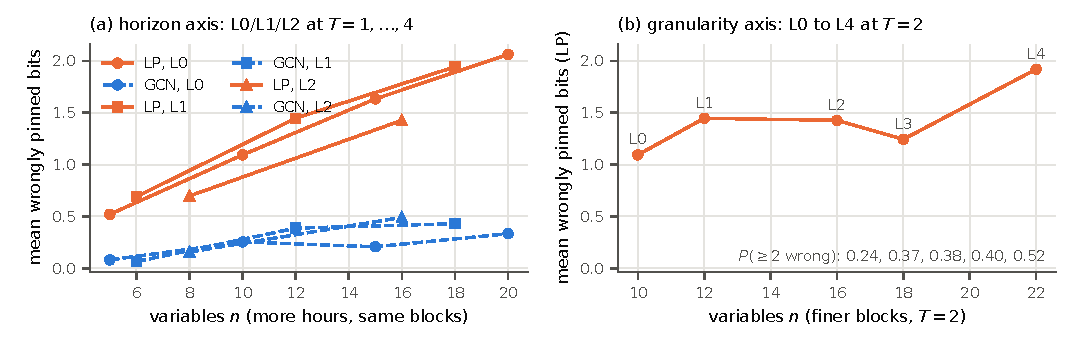
\includegraphics[width=0.72\textwidth]{figures/fig_size.pdf}
\caption{Mean wrongly pinned bits against problem size, \NCensus\ paired demand draws per cell, each cell at its own calibrated point. (a) Horizon at fixed granularity: the LP (solid) and a GCN trained at each horizon (dashed). (b) Granularity at $T=\NHoursMain$, L0--L4 (LP).}
\label{fig:size}
\end{figure*}

\subsection{Band share explains sampling on UC, not on MaxCut}
\label{sec:res-band}

\paragraph{The fit on UC} We pooled every $p=1$ run of the $\varepsilon$ sweep with nonzero overlap (all arms and all $\varepsilon$) and fitted $P_{\KMax}$ by logistic least squares (Fig.~\ref{fig:bandshare}; Supplementary Table~S5). $\log_{10}$ overlap alone gives $R^2=\BSRtwoOverlap$, and the arms separate: the per-arm mean residuals span \BSSpreadOverlap. Adding the band mass $m_5$ gives $R^2=\BSRtwoBand$, cuts the residual spread to \BSSpreadBand, and leaves nothing for arm-specific intercepts ($\Delta R^2=\BSdRtwoBand$). The coefficient on $\log_{10}m_5$ is \emph{negative} (\BSCoefBand, against \BSCoefOverlap\ on $\log_{10}$ overlap): at fixed overlap, more initial mass on other near-ground states means lower ground-state sampling.

\paragraph{Held-out checks on UC} Fitted only on the non-learned runs, overlap alone under-predicts the learned arms by \BSHeldOutOverlapMin--\BSHeldOutOverlapMax; overlap plus band mass predicts them within \BSHeldOutBandMax. Leaving out one structural group at a time, the cross-validated $R^2$ is \BSLogoOverlap\ for overlap alone and \BSLogoBand\ with band mass. At L4 the refit gives \BSLfourBand\ (overlap alone: \BSLfourOverlap), and the L2 curve applied \emph{unchanged} to L4 gives $R^2=\BSTransferBand$, against \BSTransferOverlap\ for the transferred overlap-only curve.

\paragraph{No transfer to MaxCut} The same curve applied unchanged to MaxCut fails: $R^2=\MCTransferTwelve$, \MCTransferSixteen\ and \MCTransferTwenty\ at $n=\MCSizeTwelve$, \MCSizeSixteen\ and \MCSizeTwenty\ (Table~\ref{tab:maxcut}). Refitted there, overlap alone already gives \MCOvTwelve, \MCOvSixteen\ and \MCOvTwenty, and band mass raises this to \MCBandTwelve, \MCBandSixteen\ and \MCBandTwenty, with source-specific residuals remaining. At $n=\MCSizeTwelve$ the band holds only the maximum cuts, so band share and overlap coincide. Band density does not explain the difference: across the \BDInstances\ instances of both classes it correlates with the improvement from the band (rank correlation \BDPooled), but within classes it does not (\BDWithin). Band share is a diagnostic for unit commitment; computing it needs the full spectrum.

\begin{figure*}[t]
\centering
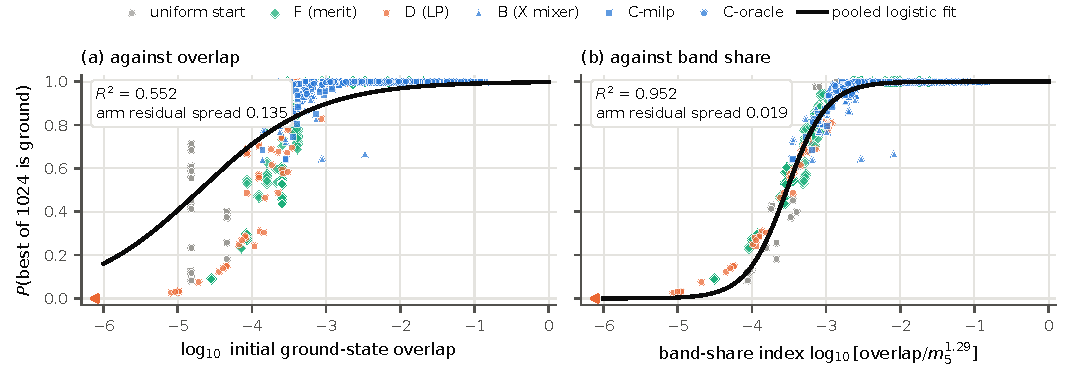
\includegraphics[width=0.72\textwidth]{figures/fig_bandshare.pdf}
\caption{UC, L2, $p=1$: $P_{\KMax}$ against (a) the initial ground-state overlap and (b) the band-share index $\log_{10}(\mathrm{overlap}/m_5^{k})$, $k=\BSExponent$ fitted. Points: arm $\times$ $\varepsilon$ $\times$ scenario means; curves: one logistic fit pooled over all arms and $\varepsilon$. On overlap the arms separate; on band share they collapse onto one curve.}
\label{fig:bandshare}
\end{figure*}

\subsection{Overlap ranks sources well and chooses $\varepsilon$ badly}
\label{sec:res-eps}

\paragraph{Ranking sources} Earlier work ranks warm starts by depth-zero quantities: initial overlap and initial approximation ratio~\cite{bhattacharyya2025qubo}. As a rule for picking the source with the highest $P_{\KMax}$ at $\varepsilon=\EpsMain$, overlap is right in \RKUCSixteenOv\ of \RKUCSixteenN\ UC instances at \NLtwo\ qubits and \RKUCTwentyTwoOv\ of \RKUCTwentyTwoN\ at \NLfour, and on every MaxCut graph where sources differ (Table~\ref{tab:maxcut}). Band share matches it on UC (\RKUCSixteenBand\ and \RKUCTwentyTwoBand) and is worse on MaxCut. The initial approximation ratio is right in only \RKUCSixteenRatio\ and \RKUCTwentyTwoRatio.

\paragraph{Choosing $\varepsilon$} A wrong $\varepsilon$ is expensive for the LP and nearly free for the learned starts (Table~\ref{tab:eps}). Measured from an arm's best $\varepsilon$ at the group level, the LP's regret is \RegretEpsFiveD\ \RegretEpsFiveDCI\ at $\varepsilon=\EpsSecond$ and \RegretEpsZeroD\ at $\varepsilon=0$, where a wrongly pinned bit can never flip. For the learned starts it is at most \RegretMaxCmilp\ (C-milp) and \RegretMaxCoracle\ (C-oracle) anywhere in $0\leq\varepsilon\leq\RegretRange$.

Choosing $\varepsilon$ per instance by maximum overlap does not remove this cost for heuristic sources, because overlap favours small $\varepsilon$. Against each instance's own best $\varepsilon$, the LP loses \ERDOvSixteen\ on average (worst instance \ERDOvWorstSixteen) and merit order \ERFOvSixteen\ (\ERFOvWorstSixteen) at \NLtwo\ qubits, and \ERDOvTwentyTwo\ (\ERDOvWorstTwentyTwo) and \ERFOvTwentyTwo\ (\ERFOvWorstTwentyTwo) at \NLfour, where the choice is between two values only. Choosing by band share loses at most \ERBandMeanMax\ on average and \ERBandWorstMax\ on one instance. For the learned starts every rule is within \ERLearnedMax\ of the best.

\begin{table*}[t]
\centering
\caption{Regularisation on UC. Each arm at its best $\varepsilon^\star$ (maximising scenario-mean $P_{\KMax}$; $\varepsilon=\EpsMax$ excluded); L2, $p=1$, \NScen\ scenarios $\times$ \NSeedsSweep\ seeds. $g$: final gain. Regret: drop in group-level $P_{\KMax}$ from $\varepsilon^\star$. Last three columns: the LP (at its own $\varepsilon^\star$) minus the arm, paired over scenarios and over the \NGroupsGL\ structural groups (95\% $t$-intervals), and group-fold cross-validated over \NSplits\ splits (mean; share of splits in which D is worse).}
\label{tab:eps}
\scriptsize
\setlength{\tabcolsep}{2.5pt}
\resizebox{\textwidth}{!}{\begin{tabular}{lcccccccccc}
\toprule
Arm & $\varepsilon^\star$ & $P_{\KMax}$ at $\varepsilon^\star$ [95\% CI] & $g$ at $\varepsilon^\star$ & $g$ at $\EpsMain$ & Regret $\varepsilon{=}0$ & Regret $\varepsilon{=}\EpsSecond$ & D $-$ arm, scenarios & D $-$ arm, GL groups & D $-$ arm, group CV \\
\midrule
C-oracle (GCN) & 0.1 & 1.000 \ensuremath{[1.000,\,1.000]} & 0.936 & 0.936 & 0.000 & 0.000 & \ensuremath{-0.100} \ensuremath{[-0.164,\,-0.036]} & \ensuremath{-0.083} \ensuremath{[-0.164,\,-0.003]} & \ensuremath{-0.094} (100\%) \\
C-milp (GCN) & 0.15 & 0.991 \ensuremath{[0.978,\,1.005]} & 0.924 & 0.936 & 0.018 & 0.010 & \ensuremath{-0.092} \ensuremath{[-0.153,\,-0.031]} & \ensuremath{-0.069} \ensuremath{[-0.140,\,+0.003]} & \ensuremath{-0.070} (96\%) \\
B (GCN, X mixer) & 0.15 & 0.994 \ensuremath{[0.985,\,1.003]} & 0.914 & 0.927 & 0.018 & 0.007 & \ensuremath{-0.094} \ensuremath{[-0.156,\,-0.032]} & \ensuremath{-0.073} \ensuremath{[-0.147,\,+0.001]} & \ensuremath{-0.079} (98\%) \\
F (merit order) & 0.25 & 0.863 \ensuremath{[0.811,\,0.915]} & 0.912 & 0.935 & 0.197 & 0.197 & \ensuremath{+0.037} \ensuremath{[-0.026,\,+0.099]} & \ensuremath{+0.047} \ensuremath{[-0.028,\,+0.122]} & \ensuremath{+0.036} (20\%) \\
\midrule
D (LP) & 0.25 & 0.900 \ensuremath{[0.836,\,0.964]} & 0.905 & 0.946 & 0.917 & 0.122 & -- & -- & -- \\
\bottomrule
\end{tabular}
}
\end{table*}

\subsection{The unit-commitment study}
\label{sec:res-arms}

\paragraph{Sources at $\varepsilon=\EpsMain$} Over \NScen\ held-out scenarios $\times$ \NSeedsMain\ seeds (Supplementary Table~S3), C-milp reaches $P_{\KMax}=\PgndCmilp$ and C-oracle \PgndCoracle; the LP reaches \PgndD, merit order (F) \PgndF, the cold start (A) \PgndA\ and the random control (E) \PgndE. Paired over scenarios, C-milp $-$ D $=\CmilpMinusD$ \CmilpMinusDCI\ (C-milp ahead in \CmilpMinusDW\ of \CmilpMinusDN), C-milp $-$ F $=\CmilpMinusF$ \CmilpMinusFCI\ and C-milp $-$ A $=\CmilpMinusA$ \CmilpMinusACI.

At the group level ($n=\NGroupsGL$), C-milp $-$ F and C-milp $-$ A keep intervals clear of zero (\CmilpMinusFGL\ \CmilpMinusFGLCI\ and \CmilpMinusAGL\ \CmilpMinusAGLCI). C-milp $-$ D is \CmilpMinusDGL\ \CmilpMinusDGLCI, an interval that touches zero: the effect against D is large in a minority of structures and zero in the rest (Section~\ref{sec:res-pins}).

Exact ground-state labels buy nothing over MILP labels (C-oracle $-$ C-milp $=\CoracleMinusCmilp$ \CoracleMinusCmilpCI). The learned state with the $X$ mixer (B) ties C-milp on $P_{\KMax}$ but is worse on single-shot $P_1$ ($\PoneBMinusCmilp$ \PoneBMinusCmilpCI). The random control is worse than starting cold (E $-$ A $=\EMinusA$ \EMinusACI). Depth barely helps the warm arms: from $p=1$ to $p=3$ C-milp moves from \PgndCmilp\ to \PgndPthreeCmilp\ and D from \PgndD\ to \PgndPthreeD.

\label{sec:res-tuned}
\paragraph{The advantage survives tuning the LP} At its own best $\varepsilon=\BestEpsD$ the LP reaches \PgndBestD\ \PgndBestCID\ (Table~\ref{tab:eps}). Paired, D $-$ C-oracle $=\BestDMinusCoracle$ \BestDMinusCoracleCI\ (group level \BestDMinusCoracleGL\ \BestDMinusCoracleGLCI), and D $-$ C-milp $=\BestDMinusCmilp$ \BestDMinusCmilpCI. At the group level the latter is \BestDMinusCmilpGL\ \BestDMinusCmilpGLCI, so granting D its in-sample best $\varepsilon$ leaves the group-level gap to C-milp borderline.

Choosing $\varepsilon$ on the scenarios it is evaluated on flatters the arm whose optimum is noisiest. Our primary numbers therefore choose $\varepsilon$ on half of the structural groups and evaluate on the other half, over \NSplits\ random splits: D $-$ C-oracle $=\CVDMinusCoracle$ (D worse in \CVDMinusCoracleWorse\% of splits), D $-$ C-milp $=\CVDMinusCmilp$ (\CVDMinusCmilpWorse\%), and D $-$ F $=\CVDMinusF$, so at its best the LP is indistinguishable from merit order.

\paragraph{Approximation ratio and sampling disagree} At $\varepsilon=\EpsMain$ the LP has the highest final gain of any arm (\GfinalD, against \GfinalCoracle\ for C-oracle), higher than C-oracle in all \GfinalCoracleMinusDL\ scenarios, while sampling the ground state less reliably in \CoracleMinusDW\ of \CoracleMinusDN. At each arm's own best $\varepsilon$ the gain order reverses, because the LP's sampling optimum lies at a larger $\varepsilon$, which moves the initial state towards uniform: the LP gives up gain to dilute its wrongly pinned bits.

\paragraph{At \NLfour\ qubits} Over \LfourNStruct\ structurally distinct L4 instances $\times$ \NSeedsLfour\ seeds at L4's own operating point (Supplementary Table~S4), C-milp $-$ D $=\LfourOwnCmilpMinusDTen$ \LfourOwnCmilpMinusDTenCI\ per structure at $\varepsilon=\EpsMain$ (C-milp ahead in \LfourOwnCmilpMinusDTenW\ of \LfourNStruct), and \LfourOwnCmilpMinusDTenRw\ \LfourOwnCmilpMinusDTenRwCI\ reweighted to the demand distribution. At the frozen point it is \LfourFrzCmilpMinusDTen\ \LfourFrzCmilpMinusDTenCI; the paired change between the two points is \LfourChangeTen\ \LfourChangeTenCI, consistent with zero though wide. Every arm does worse than at \NLtwo\ qubits: C-milp reaches \LfourOwnPgndCmilp, D \LfourOwnPgndD\ and the cold start \LfourOwnPgndA.

\label{sec:res-robust}
\paragraph{Robustness} With \ShotsMin-shot expectation estimates (Supplementary Table~S7), C-milp loses \ShotLossCmilp\ in $P_{\KMax}$, the LP \ShotLossD, the cold start \ShotLossA\ and merit order \ShotLossF. The learned start's advantage over the LP does not change significantly (\ShotAdvChange\ \ShotAdvChangeCI). Under shot noise COBYLA stops early, so this is a lightly optimised regime. Nelder--Mead with exact expectations gives C-milp $-$ D $=\NMCmilpMinusD$ \NMCmilpMinusDCI, against \ExactThreeSeedCmilpMinusD\ with COBYLA on the same runs.

\subsection{Negative results}
\label{sec:res-neg}

\paragraph{The learned start fails below its training range} We applied the unchanged L2 GCN to new conditions, \OODNScen\ scenarios $\times$ \NSeedsOOD\ seeds per test set (Supplementary Table~S8). Below the training demand range the learned start is worse than the LP: its wrong pins rise to \OODLowWrongC\ per instance (LP \OODLowWrongD), and its $P_{\KMax}$ falls to \OODLowC\ against \OODLowD: C-milp $-$ D $=\OODLowDiff$ \OODLowDiffCI, with C-milp behind in \OODLowDiffL\ of \OODNScen\ scenarios. With a changed hourly profile it falls to LP level (flat: \OODFlatC\ against \OODFlatD; reversed: \OODRevC\ against \OODRevD). A forced outage, which changes the graph, does not break it: it keeps $P_{\KMax}$ between \OODOutMin\ and \OODOutMax, at or above the LP. The LP has no training distribution to fall out of, which is a genuine advantage.

\paragraph{All warm starts are equivalent on cost} The learned starts sample the ground state more often, but their best-of-\KMax operating cost is no better than the LP's. At L2, C-milp $-$ D in repaired cost gap is \GapCmilpMinusD\ percentage points \GapCmilpMinusDCI\ at the scenario level and \GapCmilpMinusDGL\ \GapCmilpMinusDGLCI\ at the group level; at L4 it is \LfourFrzGapCmilpMinusD\ \LfourFrzGapCmilpMinusDCI\ (frozen point) and \LfourOwnGapCmilpMinusD\ \LfourOwnGapCmilpMinusDCI\ (own point). When the LP misses the ground state, it lands on a near-optimal adequate schedule.

\paragraph{A classical sampler solves these instances in milliseconds} Simulated annealing on the identical QUBO, compiled, with every returned state checked against the brute-force energy vector (Supplementary Table~S9), reaches $P(\text{ground})=\SAPgndLtwoEFive$ in \SAmsLtwoEFive\,ms at $n=\NLtwo$, against QAOA C-milp's \QAOAPgndLtwo\ in \QAOATimeLtwo\,s of simulation, and \SAPgndLfourESix\ in \SAmsLfourESix\,ms at $n=\NLfour$, against \QAOAPgndLfour\ in \QAOATimeLfour\,s. Tabu search given QAOA's wall time reaches \TabuPgndLtwo\ and \TabuPgndLfour. Only when SA is limited to the number of objective evaluations QAOA's optimiser makes, a counting generous to QAOA, does QAOA win (SA: \SAPgndEvalLtwo\ and \SAPgndEvalLfour). Both classical baselines were lightly tuned in their own favour. On MaxCut the cold start alone returns a maximum cut with probability \MCColdTwelve\ and \MCColdSixteen\ at $n=\MCSizeTwelve$ and \MCSizeSixteen, and at $n=\MCSizeTwenty$ it does better than the Goemans--Williamson start at $\varepsilon=\EpsMain$ (\MCColdTwenty\ against \MCGWTwenty): warm-starting is no advantage on that benchmark at these sizes.


\section{Discussion and limitations}
% TO WRITE.

% \bibliographystyle{IEEEtran}
% \bibliography{refs}

\end{document}
